% Author: Joel Scarinius Stävmo, Oskar Sundberg, Linus Savinainen, Samuel Wallander Leyonberg  and Gustav Pråmell
% Update: October 1, 2024
% Version: 1.0.0
% License: Apache 2.0

The following results are presented using graphs to illustrate key insights from the experiments conducted. The blue line and text represents the simplest crossover method, that swaps the last halves of two parents to create two children described in \ref{par:swap last halves}. The red represents the second crossover method, which selects genes from each parent based on their fitness scores, detailed in \ref{par:swap single genes}. The orange represents the third crossover method, that selects contiguous gene segments from each parent based on their fitness scores, outlined in \ref{par:swap sequnce of genes}.

\subsection{Building Small}
Figure \ref{fig:Building Small results} presents the results for 100 people in the building, as well as the worst performance from five runs for each crossover on the smallest building configuration with 10 people. Figure \ref{fig:Building Small worst} displays the worst case in these runs where the blue crossover failed to serve one person and incurred a large penalty. To highlight that with more people in a building, the orange crossover kept getting good results with great consistency Figure \ref{fig:Building Small 100 people} was used. The blue acted comparably, but it wasn't as consistent. The red one was highly unreliable, occasionally achieved positive results on the other hand, it frequently got stuck in local minimums for extended durations. Besides that it took more generations for all crossovers to reach an acceptable solution because of the increased number of people. The orange and blue crossover often reached a good solution quicker than the red one, which also tends to get worse the more people it has to serve.

\begin{figure}[ht]
	\centering
	\begin{subfigure}[b]{0.49\linewidth}
		\centering
		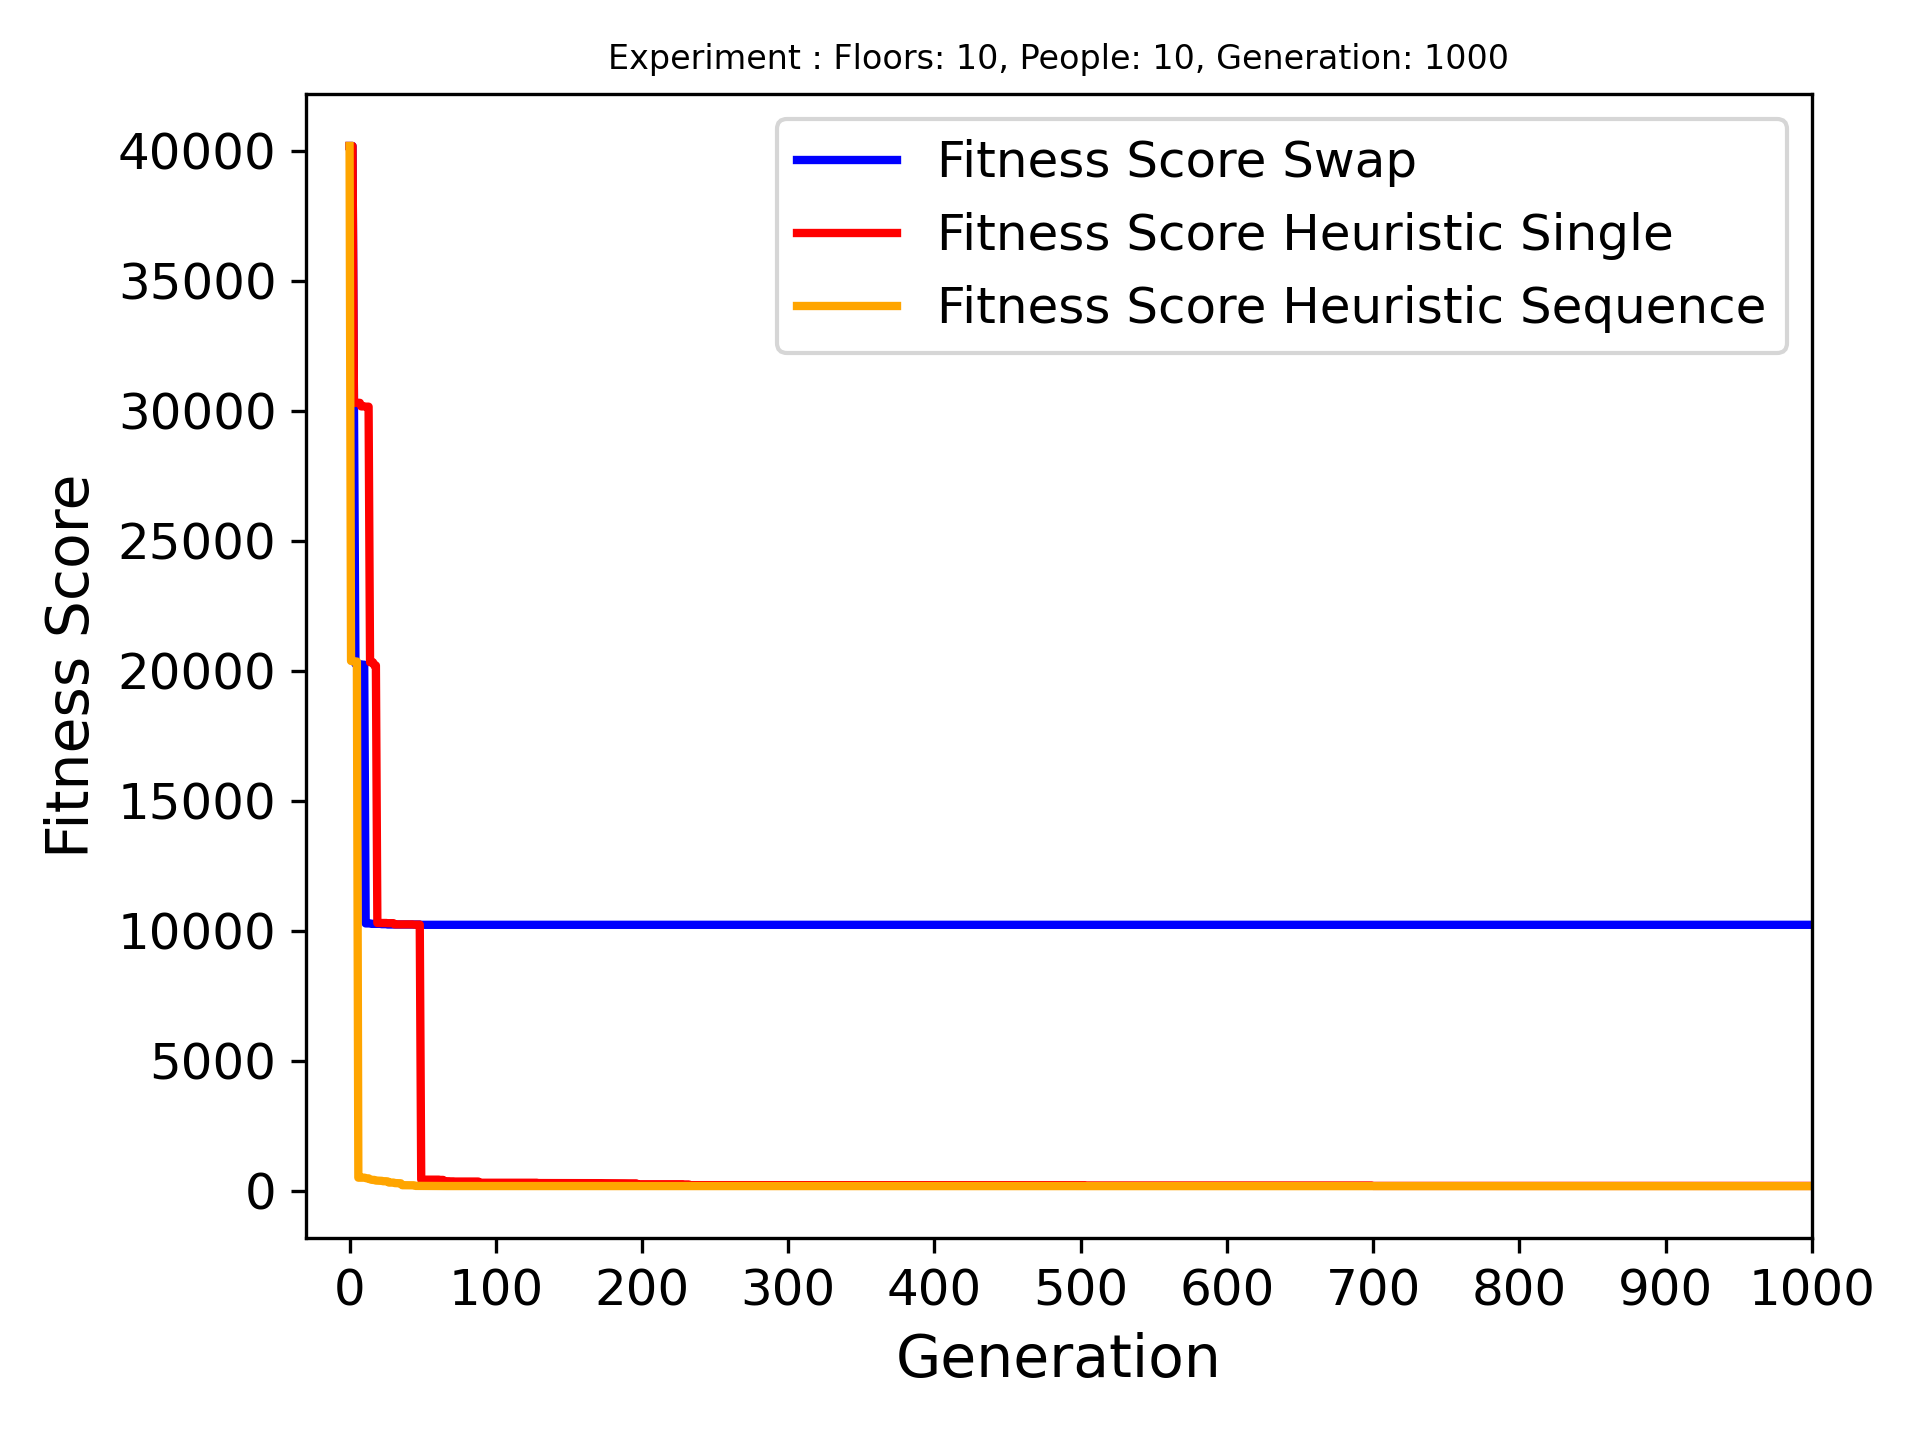
\includegraphics[width=\linewidth]{results/Building_Small/Mutation_0.1/Floors__10,_People__10,_Generation__1000_worst.png}
		\captionsetup{justification=centering,font=tiny}
		\caption{Score/Arrived/Length:\\\textcolor{blue}{10227/9/9}, \textcolor{red}{182/10/11}, \textcolor{orange}{172/10/11}.}
		\label{fig:Building Small worst}
	\end{subfigure}
	\hfill
	\begin{subfigure}[b]{0.49\linewidth}
		\centering
		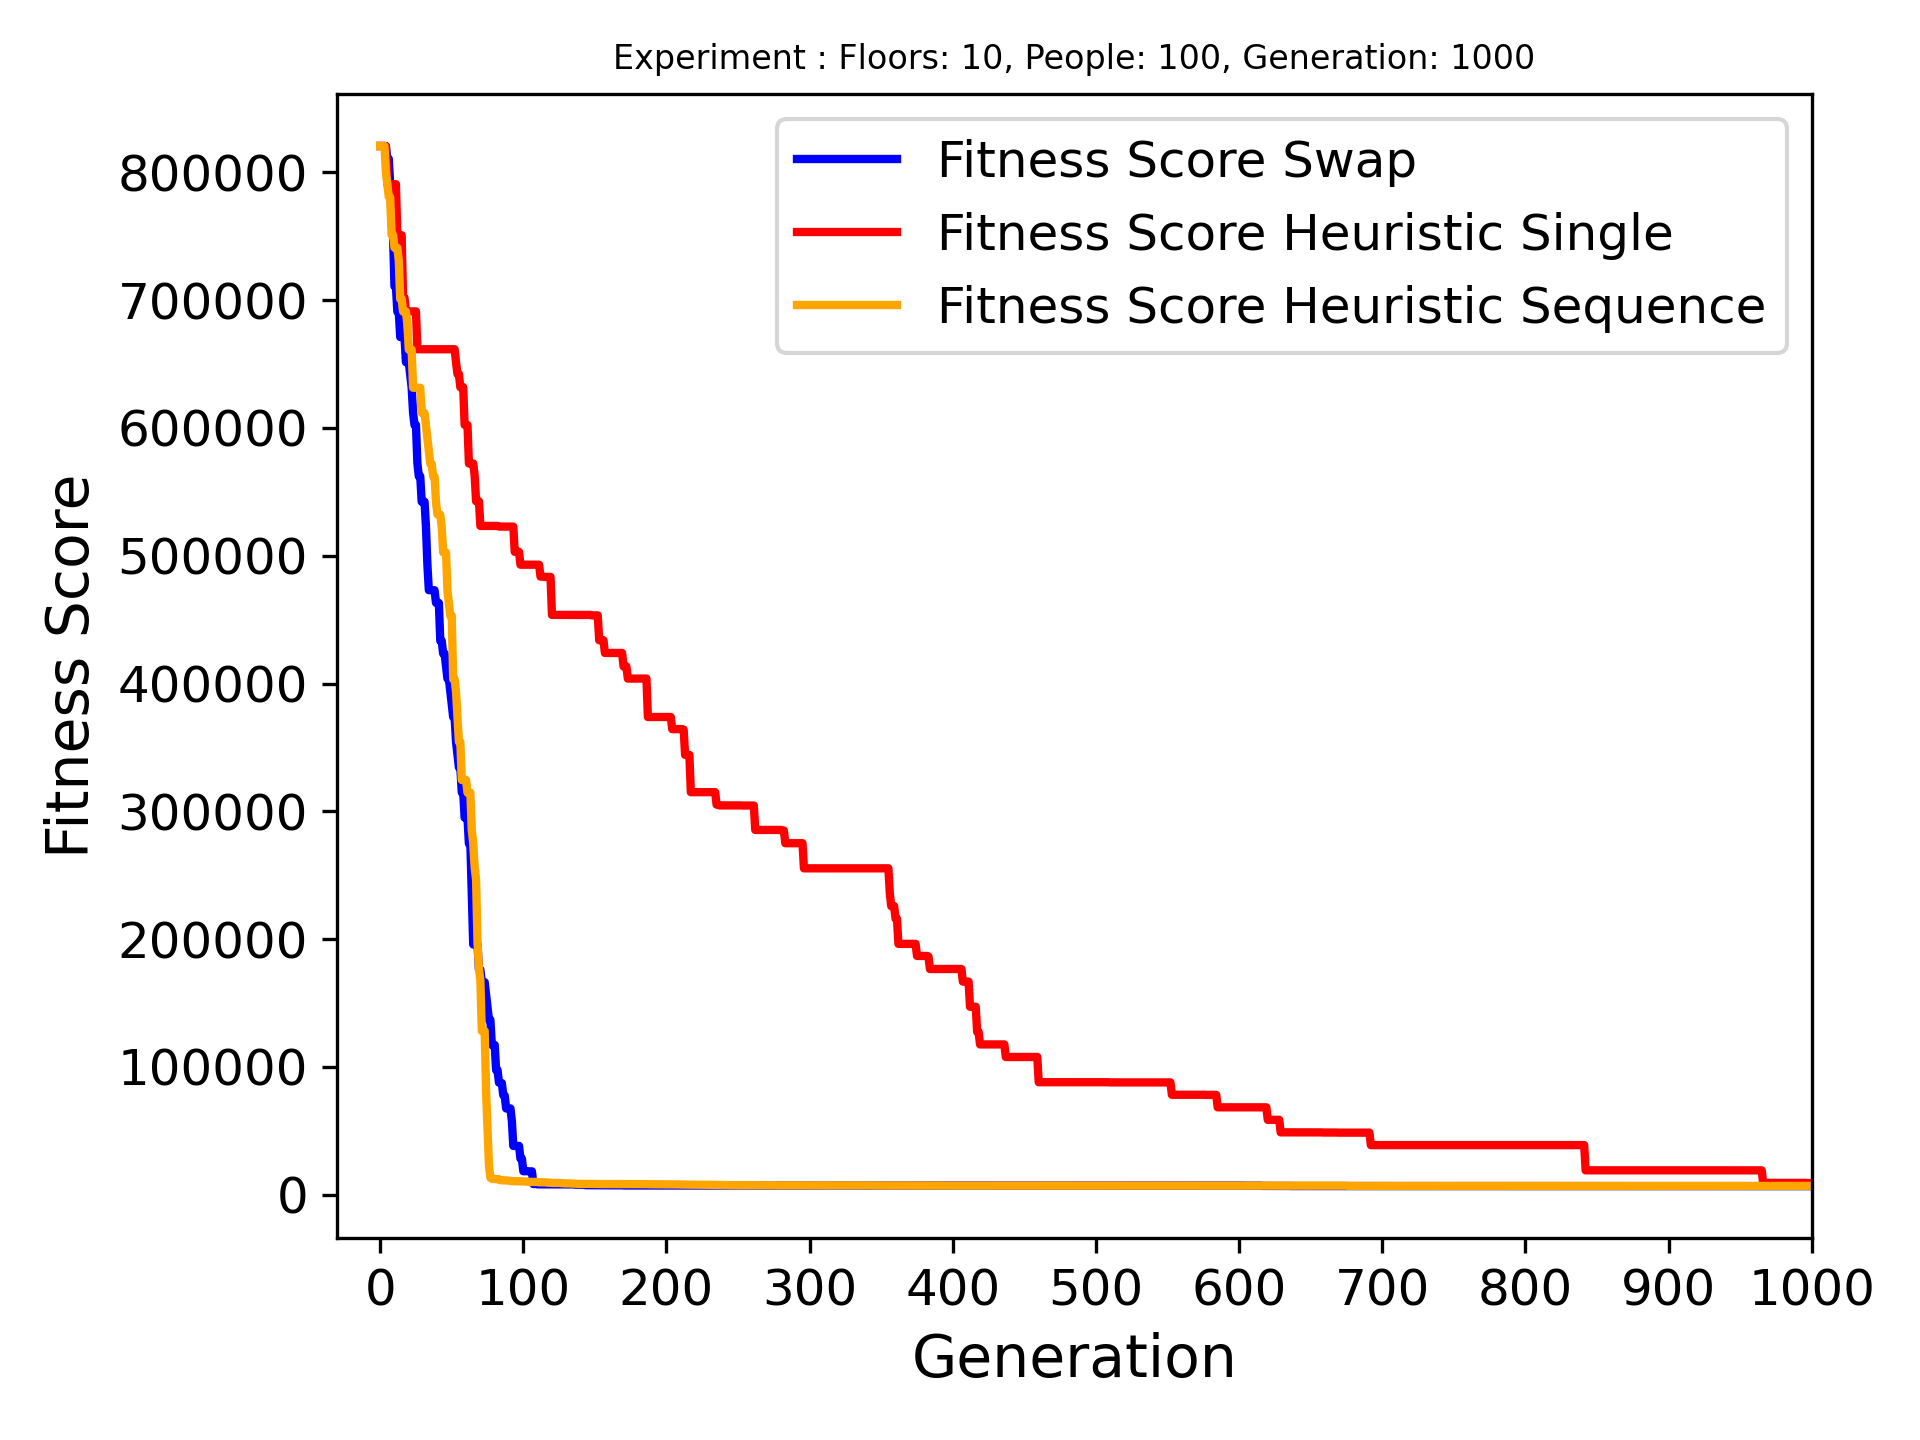
\includegraphics[width=\linewidth]{results/Building_Small/Mutation_0.1/Floors__10,_People__100,_Generation__1000.png}
		\captionsetup{justification=centering,font=tiny}
		\caption{Score/Arrived/Length:\\\textcolor{blue}{6727/100/45}, \textcolor{red}{9113/100/61}, \textcolor{orange}{6880/100/52}.}
		\label{fig:Building Small 100 people}
	\end{subfigure}
	\captionsetup{font=scriptsize}
	\caption{Comparing worst and best case.}
	\label{fig:Building Small results}
\end{figure}

\newpage

\subsection{Building Medium}
As previously noted, the red crossover tends to perform worse the more people in the building instances and Figure \ref{fig:Building Medium results} illustrates this once again. In Figure \ref{fig:Building Medium worst} the blue crossover outperformed the orange one, that got stuck in a local minimum for an extended period. The orange crossover was also slower than the blue one. Conversely, Figure \ref{fig:Building Medium best} then shows a scenario where the blue one performed similarly to how it performed in \ref{fig:Building Medium worst} and the orange one reached an extraordinary low score of 121157 without getting stuck in a local minimum. This demonstrates that the orange crossover have both strong worst case and great best case. This further underlines that the orange crossover is the most reliable crossover of the three.

\begin{figure}[ht]
	\centering
	\begin{subfigure}[b]{0.49\linewidth}
		\centering
		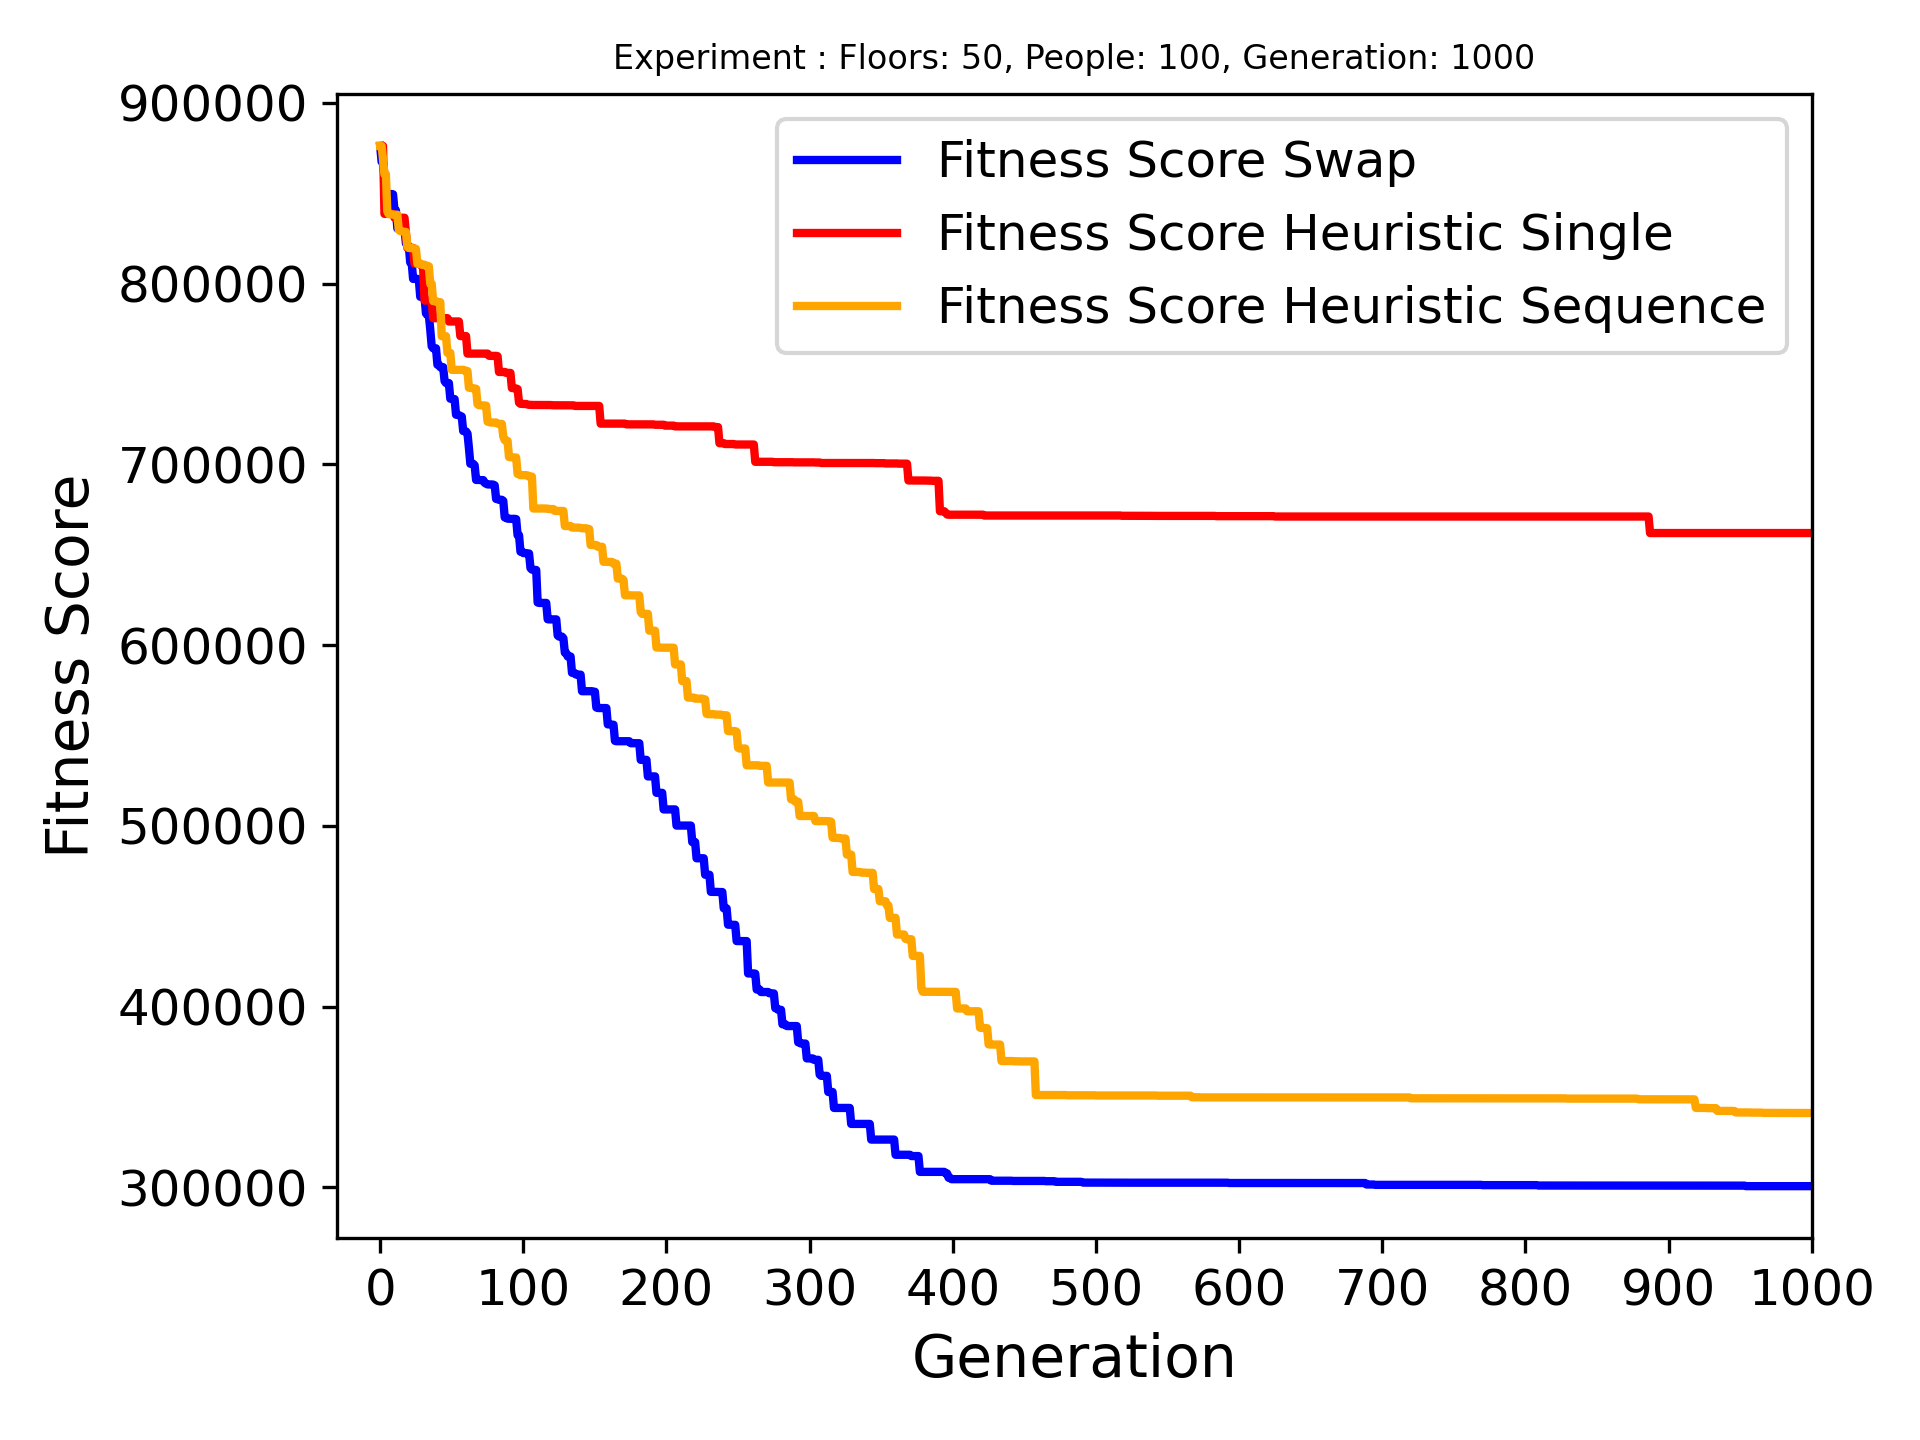
\includegraphics[width=\linewidth]{results/Building_Medium/Mutation_0.1/Floors__50,_People__100,_Generation__1000_4_worst.png}
		\captionsetup{justification=centering,font=tiny}
		\caption{Score/Arrived/Length:\\\textcolor{blue}{300697/74/69}, \textcolor{red}{661991/35/52}, \textcolor{orange}{341167/69/74}.}
		\label{fig:Building Medium worst}
	\end{subfigure}
	\hfill
	\begin{subfigure}[b]{0.49\linewidth}
		\centering
		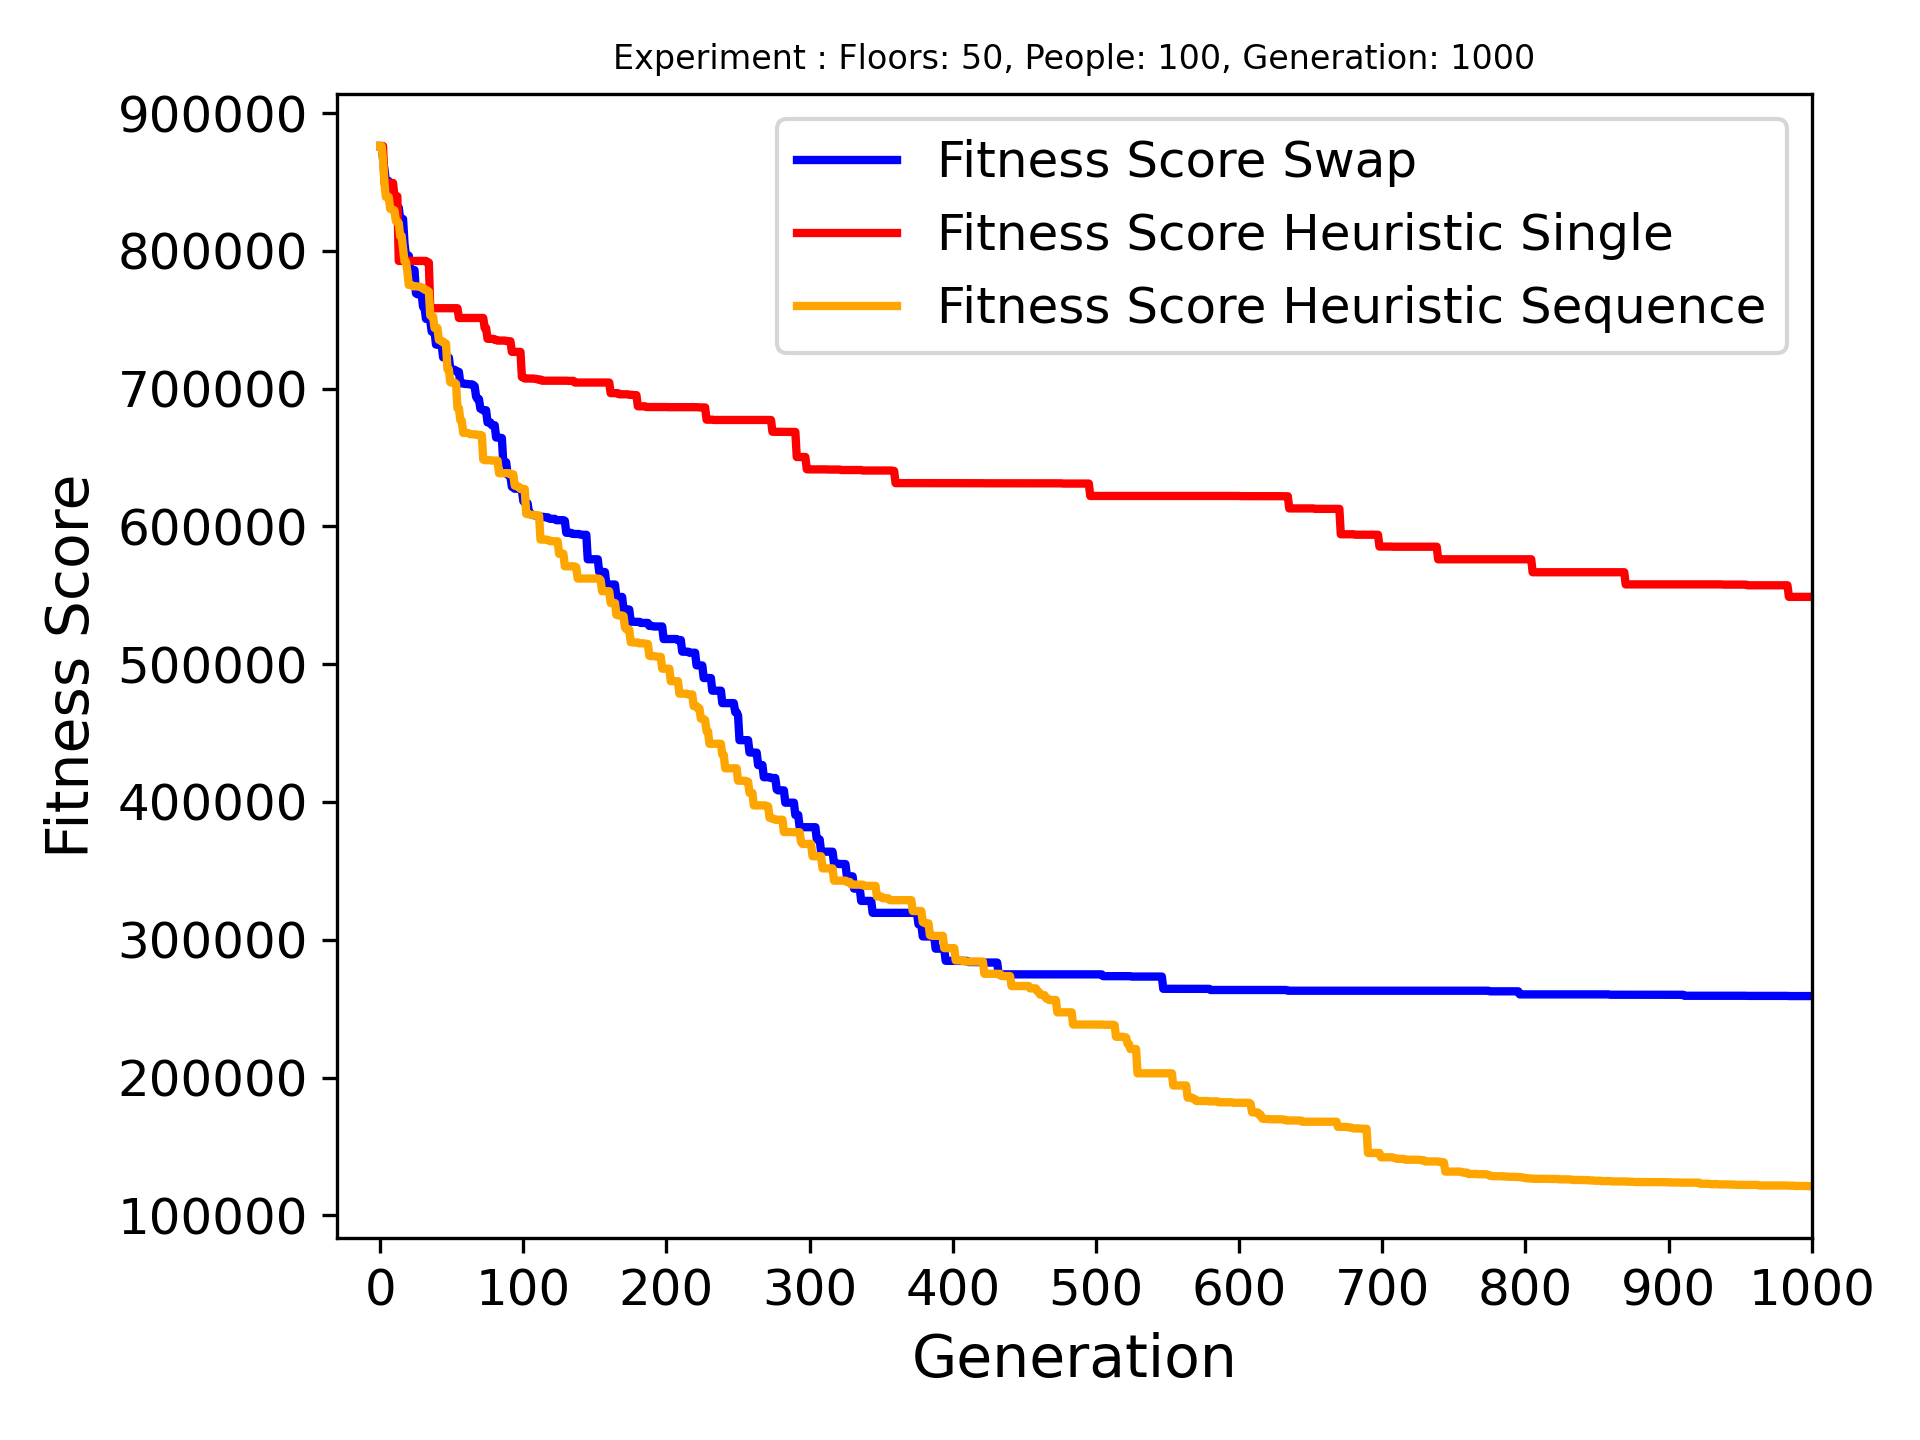
\includegraphics[width=\linewidth]{results/Building_Medium/Mutation_0.1/Floors__50,_People__100,_Generation__1000_1_best.png}
		\captionsetup{justification=centering,font=tiny}
		\caption{Score/Arrived/Length:\\\textcolor{blue}{259130/79/71}, \textcolor{red}{548857/48/59}, \textcolor{orange}{121157/94/124}.}
		\label{fig:Building Medium best}
	\end{subfigure}
	\captionsetup{font=scriptsize}
	\caption{Comparing worst and best case.}
	\label{fig:Building Medium results}
\end{figure}

\newpage

\subsection{Building Large}
After running all the buildings with a 10\% mutation rate, numerous experiments were executed with different rates. It was quickly determined that an increased mutation rate enabled the algorithm to find solutions that served all or almost all people much faster. Results in Figure \ref{fig:Building Large results} shows the best runs with mutation rates of 10\% and 60\%.

With a low mutation rate as in Figure \ref{fig:Building Large 0.1 best}, the best solutions achieved fitness scores around 500 000, whereas a higher rate tested in Figure \ref{fig:Building Large 0.6 best} yielded scores around 200 000. In the best run with a 10\% mutation rate, 66 people were served and the best run with a 60\% mutation rate served all 100 people. Not only that, it is clear that the algorithm reached acceptable solutions in a greater pace than before. Reason behind this is that to be able to serve as many people as possible the genomes have to mutate to become longer than number of floors. The higher mutation rate allowed the algorithm to reach this objective and escape local minimums faster. Further experimentation with mutation rates could potentially yield even better outcomes.

Similar results were obtained by increasing the number of generations and population size. The downside with this is that it requires more computational power and takes longer time to run. Therefore, a greater mutation rate was beneficial for fast feedback and limited hardware resources.

\begin{figure}[ht]
	\centering
	\begin{subfigure}[b]{0.49\linewidth}
		\centering
		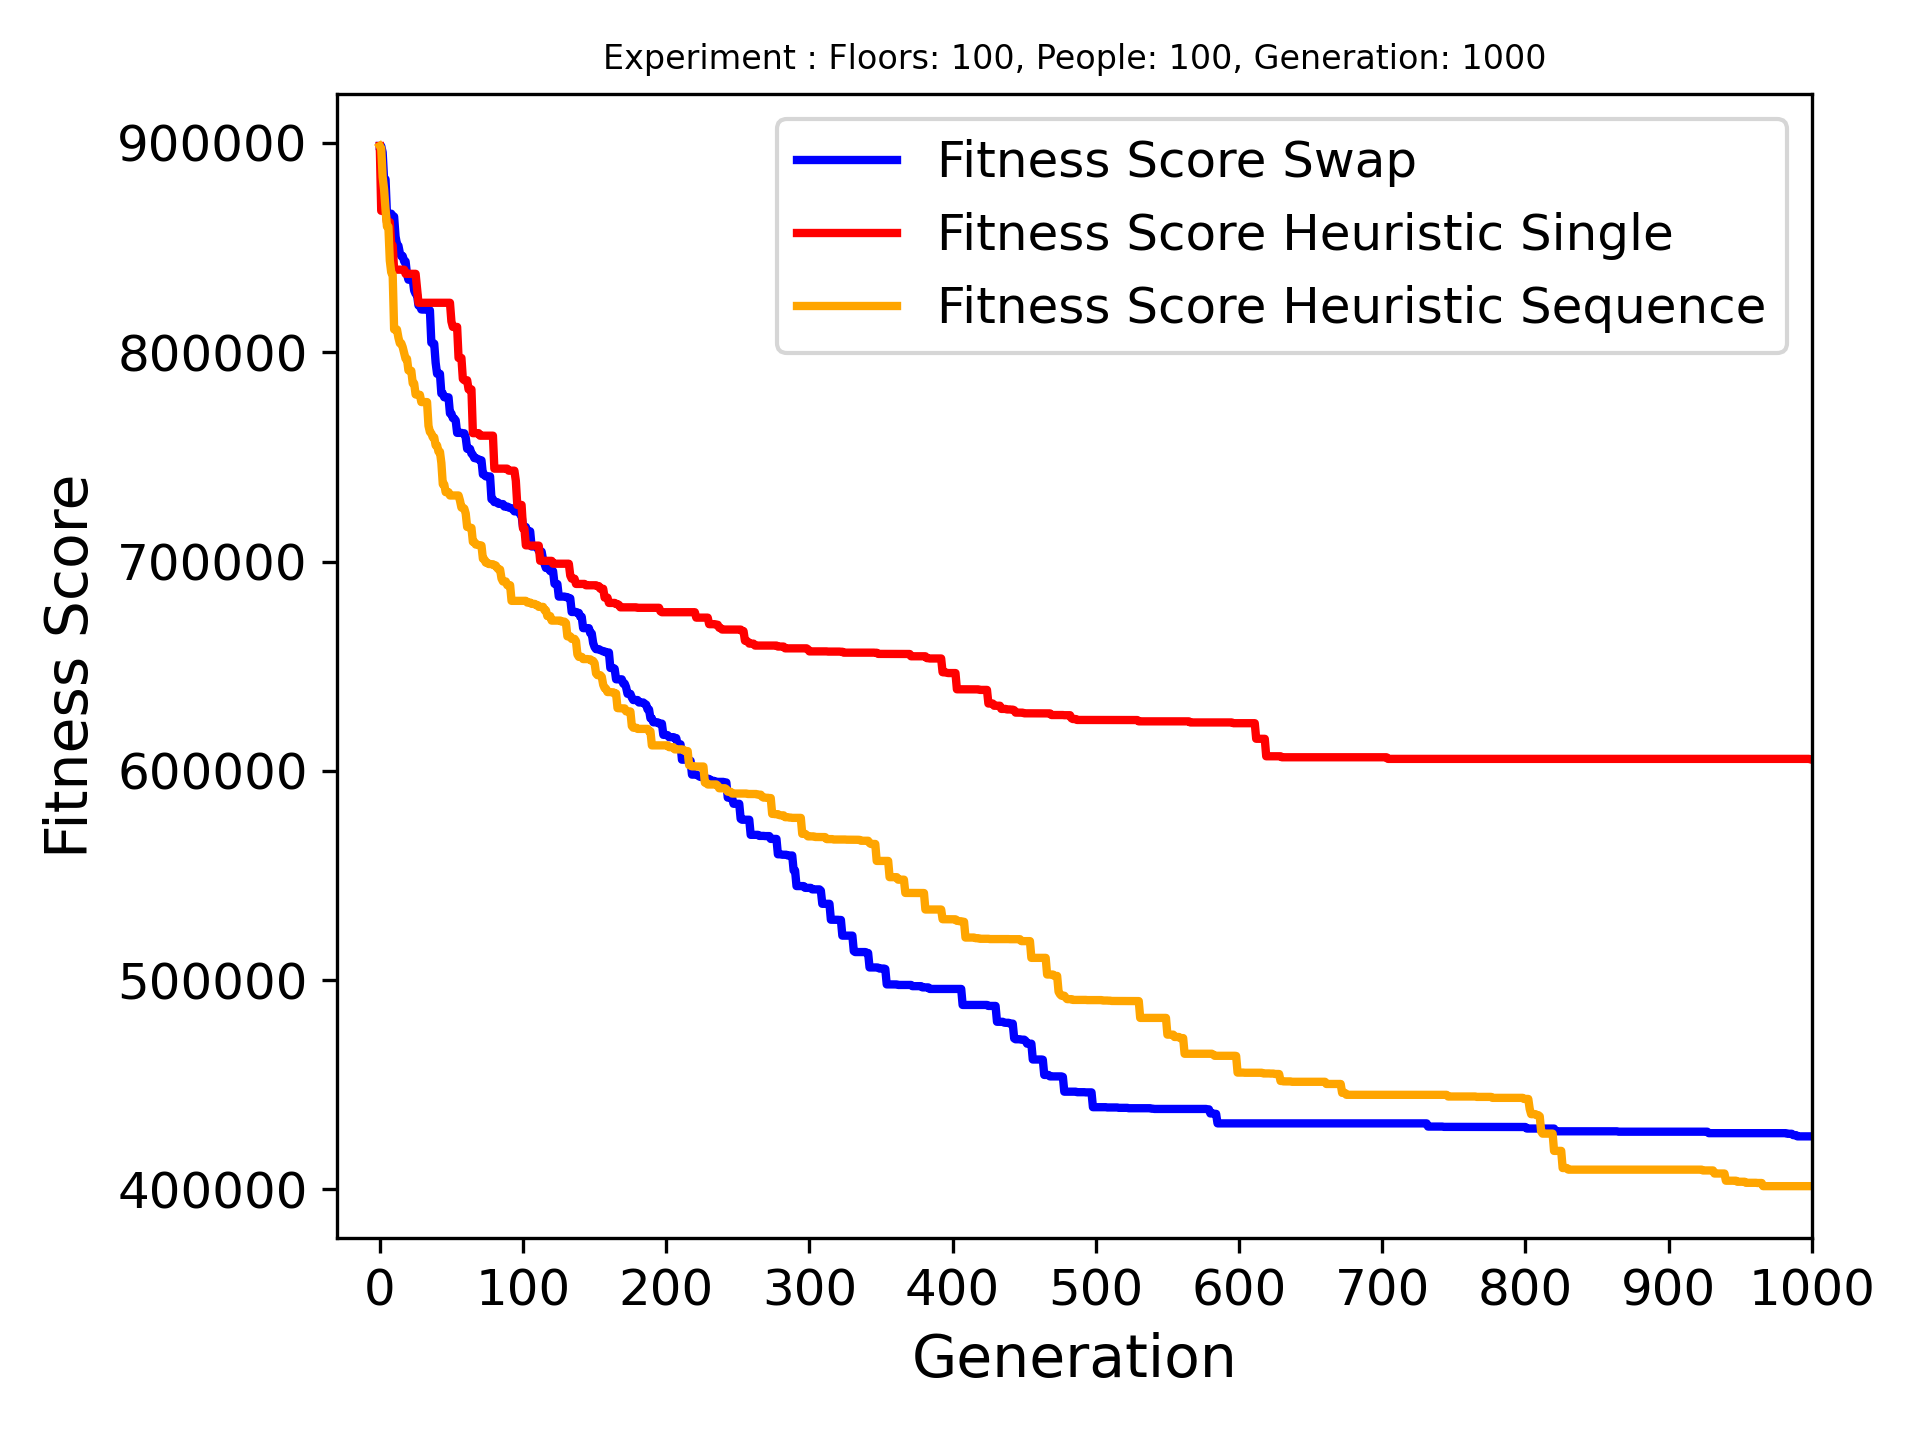
\includegraphics[width=\linewidth]{results/Building_Large/Mutation_0.1/Floors__100,_People__100,_Generation__1000_2_best.png}
		\captionsetup{justification=centering,font=tiny}
		\caption{Score/Arrived/Length:\\\textcolor{blue}{425352/67/80}, \textcolor{red}{605508/44/102}, \textcolor{orange}{401562/66/75}.}
		\label{fig:Building Large 0.1 best}
	\end{subfigure}
	\hfill
	\begin{subfigure}[b]{0.49\linewidth}
		\centering
		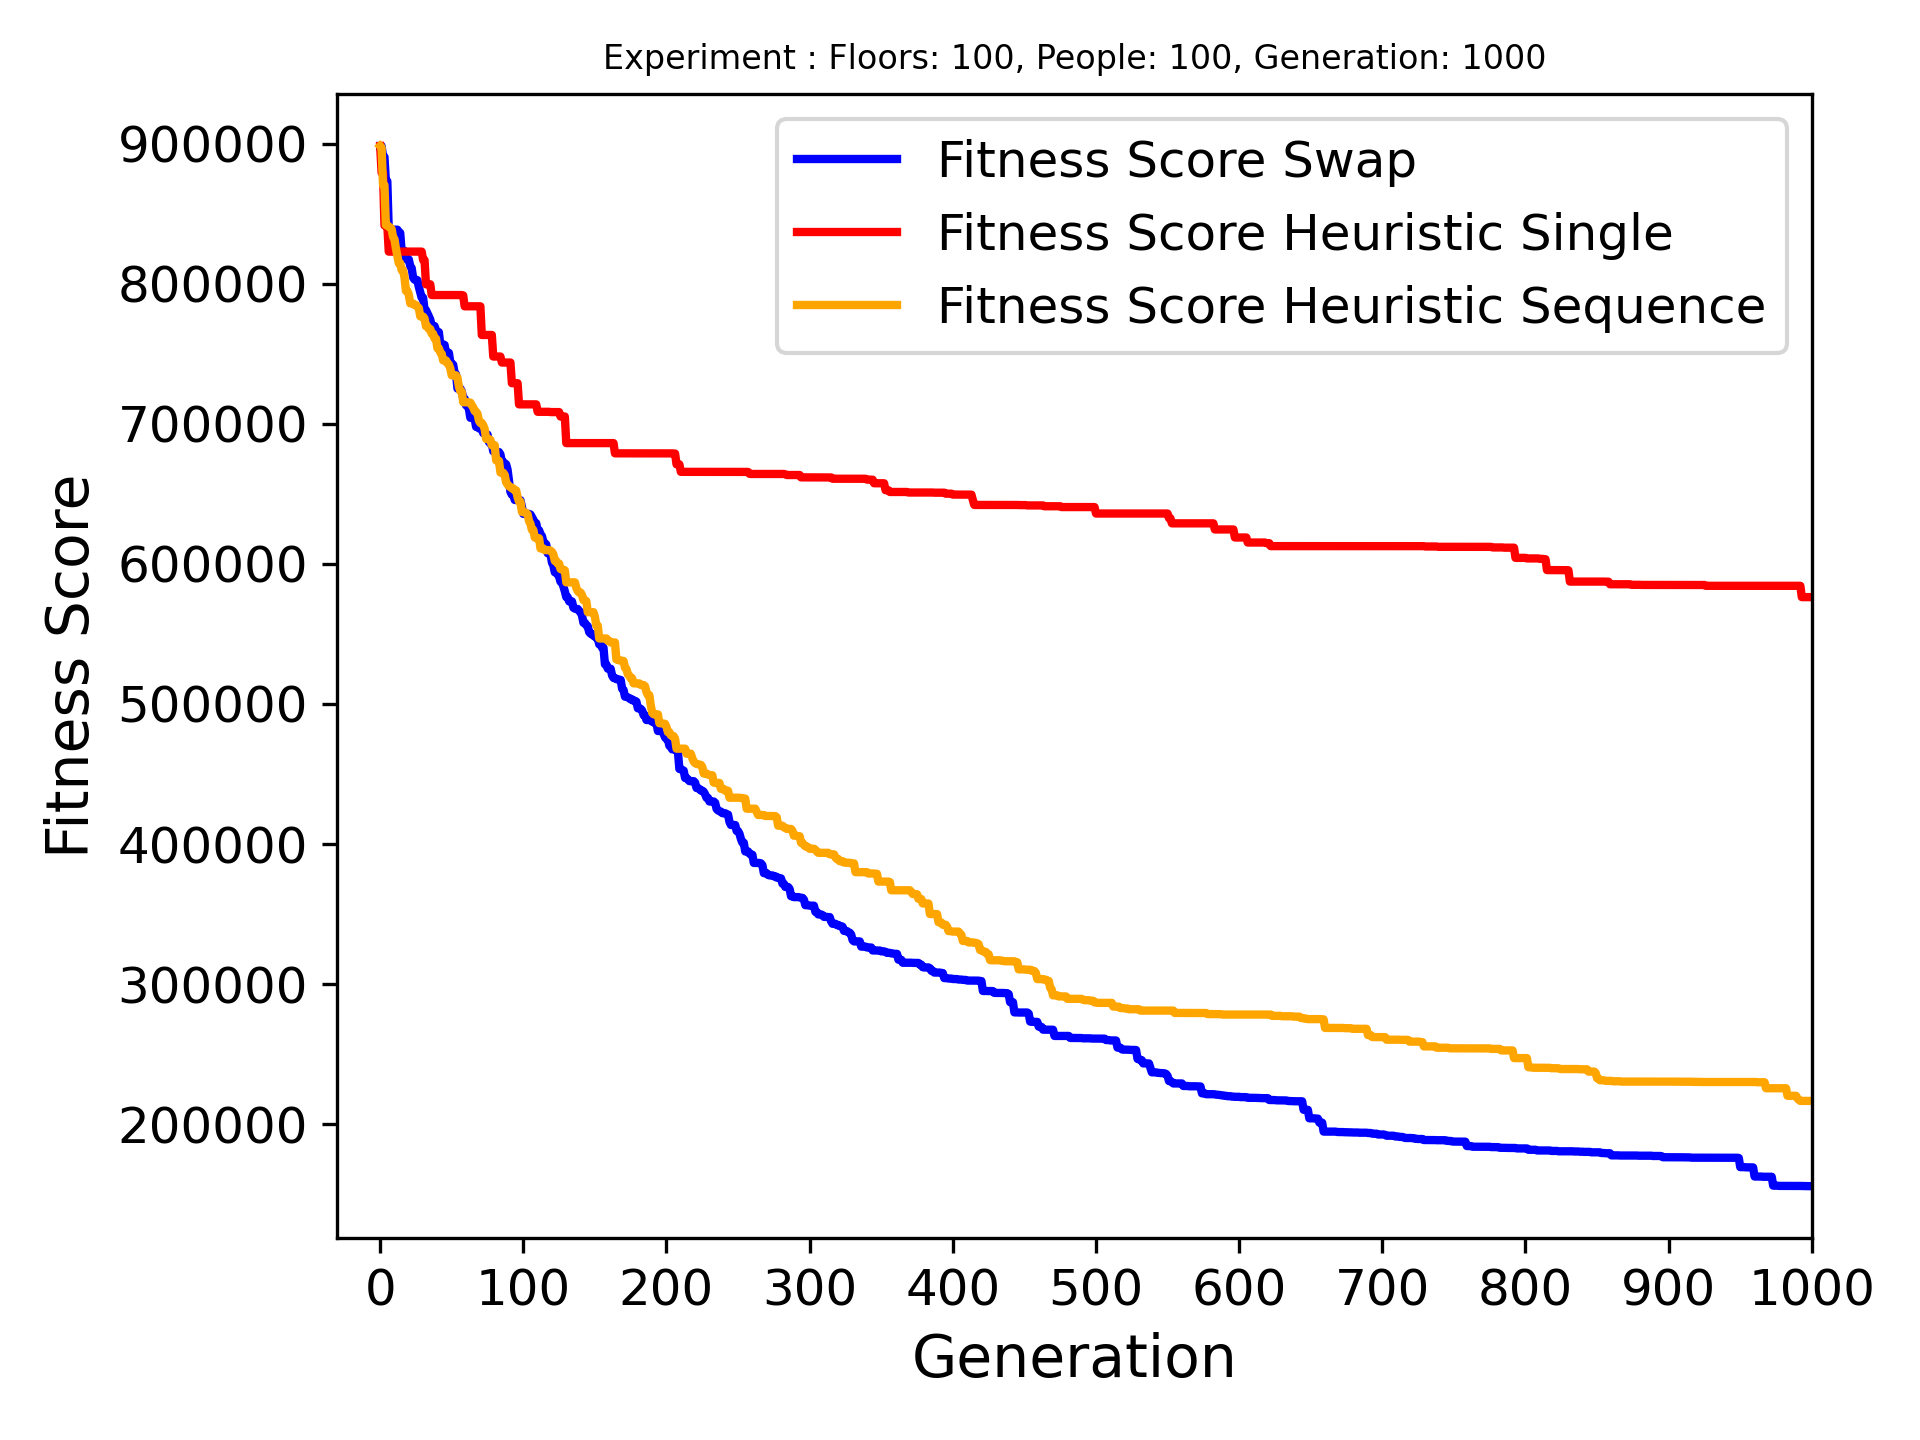
\includegraphics[width=\linewidth]{results/Building_Large/Mutation_0.6/Floors__100,_People__100,_Generation__1000_best.png}
		\captionsetup{justification=centering,font=tiny}
		\caption{Score/Arrived/Length:\\\textcolor{blue}{155619/100/151}, \textcolor{red}{576322/48/117}, \textcolor{orange}{216508/94/139}.}
		\label{fig:Building Large 0.6 best}
	\end{subfigure}
	\captionsetup{font=scriptsize}
	\caption{Comparing the best case for 10\% and 60\% mutation rate.}
	\label{fig:Building Large results}
\end{figure}

\newpage

\subsection{Building Special}
This special building used in experiments replicates the setup from a prior investigation on optimization techniques for the elevator dispatching problem \cite{gharieb2005optimal}. The people in this building has identical starting floors and destinations as the referenced study. Parameters for elevator population and number of generations are also aligned with values used for experimentation in the paper. This was done to ensure a fair comparison between the research. A minor difference is that the fitness function used in this study also gives an extra penalty for each extra floor a person travels in the elevator, as detailed in \ref{subsec:fitness_function}. Furthermore, the mutation used in this study also allows the genome length to increase and decrease.

The genetic algorithm in \cite{gharieb2005optimal} utilized Davis-order crossover, swap mutation, elitism, and a fitness function that measured the average time for all passengers to reach desired floor. The average result reported from running described algorithm, based on 5 runs was 279.1 seconds per traveler. In comparison, the average result in this study for 5 runs, was 305.1 seconds. Thus, this algorithm was approximately 26 seconds ($\approx$ 8.5\%) slower than the result in the paper. This difference could be explained by the extra penalty given in the fitness function. Additionally, it is possibly a coincidence, but one factor might have been that Davis-order crossover divides the chromosome into more segments while this crossover only splits it into two larger segments. Why this might affect the result is because when splitting the parent chromosome into two larger segments, parts of them will probably not contribute to a better result, and they will have a larger risk of remaining throughout more generations.